%%%%%%%%%%%%%%%%%%%%%%%%%%%%%%%%%%%%%%%%%
% Fancyslides Presentation
% LaTeX Template
% Version 1.0 (30/6/13)
%
% This template has been downloaded from:
% http://www.LaTeXTemplates.com
%
% The Fancyslides class was created by:
% Paweł Łupkowski (pawel.lupkowski@gmail.com)
%
% License:
% CC BY-NC-SA 3.0 (http://creativecommons.org/licenses/by-nc-sa/3.0/)
%
%%%%%%%%%%%%%%%%%%%%%%%%%%%%%%%%%%%%%%%%%

%----------------------------------------------------------------------------------------
%	PACKAGES AND OTHER DOCUMENT CONFIGURATIONS
%----------------------------------------------------------------------------------------

\documentclass{fancyslides}
\PassOptionsToPackage{usenames}{xcolor}
%\usefonttheme[onlymath]{serif}
\usefonttheme{professionalfonts}
%\usepackage{mathpazo}
%\usepackage[T1]{fontenc}
\usepackage[utf8]{inputenc} % Allows the usage of non-english characters
%\usepackage{times} % Use the Times font
%\usepackage{pifont}
\usepackage{pgfplots}
\usepackage{subcaption}
\usepackage{draftwatermark}
\usepackage{background}
\usepackage{xcolor}
%\usepackage{MnSymbol}
\usepackage{amsmath}
\usepackage{scalerel}
\usepackage{graphicx}
\usepgfplotslibrary{fillbetween}
\usetikzlibrary{patterns}
\usetikzlibrary{intersections}
\pgfplotsset{compat=1.12}
\usepackage{bm}
\usepackage{booktabs} % Allows the use of \toprule, \midrule and \bottomrule in tables
\graphicspath{{images/}} % Location of the slide background and figure files

% Beamer options - do not change
\usetheme{default} 
\setbeamertemplate{navigation symbols}{} % Disable the slide navigation buttons on the bottom of each slide
\setbeamercolor{structure}{fg=\yourowntexcol} % Define the color of titles and fixed text elements (e.g. bullet points)
\setbeamercolor{normal text}{fg=\yourowntexcol} % Define the color of text in the presentation

%%-------------------------I ADDED THIS----------------------------------------------------------
%\setbeamertemplate{background canvas}{\begin{tikzpicture}\node[opacity=.75]{\includegraphics
%[width=1.5\paperwidth]{qubbg}};\end{tikzpicture}}
%\SetWatermarkText{\includegraphics{qubbg}}
%\backgroundsetup{%
%  scale=5,       %% change accordingly
%  angle=0,       %% change accordingly
%  opacity=.6,    %% change accordingly
%  color =black,  %% change accordingly
%  contents={\begin{tikzpicture}[remember picture,overlay]
%        \node at ([yshift=11pt,xshift=5pt]current page.center) {\includegraphics[width=5cm]{qubbg}};    %% yshift and xshift for example only
%    \end{tikzpicture}}
%}
%\setbeamertemplate{background}{\BgMaterial}
%-------------------------------------------------------------------------------------------------------
\DeclareMathOperator*{\SumInt}{%
\mathchoice%
  {\ooalign{$\displaystyle\sum$\cr\hidewidth$\displaystyle\int$\hidewidth\cr}}
  {\ooalign{\raisebox{.14\height}{\scalebox{.7}{$\textstyle\sum$}}\cr\hidewidth$\textstyle\int$\hidewidth\cr}}
  {\ooalign{\raisebox{.2\height}{\scalebox{.6}{$\scriptstyle\sum$}}\cr$\scriptstyle\int$\cr}}
  {\ooalign{\raisebox{.2\height}{\scalebox{.6}{$\scriptstyle\sum$}}\cr$\scriptstyle\int$\cr}}
}
%------------------------------------------------
% COLORS
% The following colors are predefined in this class: white, black, gray, blue, green and orange

% Define your own color as follows:
%\definecolor{pink}{rgb}{156,0,151}

\newcommand{\structureopacity}{0.0} % Opacity (transparency) for the structure elements (boxes and circles)

\definecolor{BrickRed}{rgb}{.32,0,0.5}

\newcommand{\strcolor}{blue} % Set the color of structure elements (boxes and circles)
\newcommand{\yourowntexcol}{BrickRed} % Set the text color


\newlength{\wideitemsep}
\setlength{\wideitemsep}{\itemsep}
\addtolength{\wideitemsep}{5pt}
\let\olditem\item
\renewcommand{\item}{\setlength{\itemsep}{\wideitemsep}\olditem}

%%%%%%%%%%%%%%hydrogen%%%%%%%%%%%%%%%%%%%%%%%%
\newcommand{\wfnh}{\Psi({\bf{r}},t)}
\newcommand{\brah}{\langle\ell' m'|}
\newcommand{\keth}{|\ell m\rangle}
\newcommand{\sumsh}{\sum_{\ell,m}}
\newcommand{\Fh}{\frac{F_{\ell m}(r,t)}{r}}
\newcommand{\fh}{F_{\ell m}(r,t)}
\newcommand{\fph}{F_{\ell' m'}(r,t)}
\newcommand{\ddt}{\frac{\partial}{\partial t}}

%%%%%%%%%%%%%%%%%%%%%%helium%%%%%%%%%%%%%%%%%%

\newcommand{\bra}{\langle \ell'_1 \ell'_2 L'|}
\newcommand{\ket}{|\ell_1 \ell_2 L\rangle}
\newcommand{\sums}{\sum_{\ell_1,\ell_2,L}}
\newcommand{\F}{ \frac{F_{\ell_1 \ell_2 L}(r_1, r_2, t)}{r_1 r_2} } 
\newcommand{\f}{F_{\ell_1 \ell_2 L}(r_1, r_2, t)}
\newcommand{\fp}{F_{\ell'_{\rm1} \ell'_{\rm2} L'}(r_{\rm 1}, r_{\rm 2}, t)}
\newcommand{\wfn}{\sum_{\ell_1,\ell_2,L,M}\frac{F_{\ell_1 \ell_2 LM}(r_1, r_2, t)}{r_1 r_2} |\ell_1 \ell_2 LM\rangle}
\newcommand{\wfndip}{\sum_{l_1,l_2,L}\frac{P_{l_1 l_2}^{LS}(r_1, r_2, t)}{r_1 r_2} |l_1 l_2 L\rangle}
\newcommand{\nn}{\nonumber}
\newcommand{\Iat}{I_{\rm{at}}}
\newcommand{\Iee}{I_{\rm{ee}}}
\newcommand{\Iint}{I_{\rm{int}}}
\newcommand{\Hatom}{-\frac{1}{2}\nabla_j^2 -\frac{Z}{r_j}}
\newcommand{\Hintz}{-\frac{i}{\rm{c}} A (t)\frac{\partial}{\partial z_j}}
\newcommand{\Hee}{\frac{1}{r_{12}}}
\newcommand{\Hint}{ -\frac{i}{\rm{c}} \bf{A}\it^{(\rm0)}(t)\cdot\nabla_{j}}
\newcommand{\Hndip}{\frac{1}{\rm c^2}\bf{A}\it^{(\rm0)}(t)\cdot \bf{A}\it^{(\rm1)}(\bf r_{\it j}\it,t)}
\newcommand{\nablasq}{\frac{\partial^2}{\partial r_1^2} +\frac{2}{r_1}\frac{\partial}{\partial r_1}
-\frac{\hat{\ell}_{1}^{\rm2}}{r_1^2}}
\newcommand{\A}{\bf A\it(\bf r\it, t)}
\newcommand{\Ibar}{\bar{I}}
\newcommand{\nl}{\vspace{0.1in}}
\newcommand{\bi}{\begin{itemize}}
\newcommand{\ei}{\end{itemize}}
\newcommand{\eo}{\end{overlay}}
\newcommand{\bs}{\begin{slide}}
\newcommand{\es}{\end{slide}}
\newcommand{\ef}{\end{frame}}
\newcommand{\s}{\sf\epsfslidesize\white}
\newcommand{\BRA}{\langle \ell'_1 \ell'_2 L' M'|}
\newcommand{\KET}{|\ell_1 \ell_2 L M\rangle}
\newcommand{\Wcm}{W/cm$^2$}
\newcommand{\rd}{{\rm d}}
\newcommand{\dg}{^{\circ}}
%%%%%%%%%%%%%%%%%%%%%%%%%%%%%%%%%%%%%%%%%%%%
\newcommand{\PRA}{Phys. Rev. A}
\newcommand{\PRL}{Phys. Rev. Lett.}
\newcommand{\JPB}{J. Phys. B}
%%%%%%%%%%%%%%%%%%%%%%%%%%%%%%%%%%%%%%%%%%%%
%----------------------------------------------------------------------------------------
%	TITLE SLIDE
%----------------------------------------------------------------------------------------
%
%\newcommand{\titlephrase}{A LONG AND COMPLICATED PRESENTATION TITLE} % Presentation title
%\newcommand{\name}{John Smith} % Presenter's name
%\newcommand{\affil}{UCLA} % Presenter's institution
%\newcommand{\email}{john@LaTeXTemplates.com} % Presenter's email address
%
\begin{document}
%
%\startingslide % This command inserts the title slide as the first slide
\pgfmathdeclarefunction{gauss}{3}{%
  \pgfmathparse{#3/(#2*sqrt(2*pi))*exp(-((x-#1)^2)/(2*#2^2))}%
}

\pgfmathdeclarefunction{gauss2}{6}{%
  \pgfmathparse{#3/(#2*sqrt(2*pi))*exp(-((x-#1)^2)/(2*#2^2))+#6/(#5*sqrt(2*pi))*exp(-((x-#4)^2)/(2*#5^2))}%
}

%----------------------------------------------------------------------------------------
%	PRESENTATION SLIDES
%------------------------------------------------
\fbckg{qubbg3}
\begin{frame}

\begin{center}
{\bf\large R-Matrix with time-dependence for atoms in arbitrarily-polarized laser fields}
\\ \vspace{0.1in}
\small
G. S. J. Armstrong, D. D. A. Clarke, A. C. Brown, H. W. van der Hart
\\ 
\vspace{0.1in}
Centre for Theoretical Atomic, Molecular and Optical Physics,
\\
Queen's University Belfast
\end{center}

%\small
%%\begin{center}
%G. S. J. Armstrong, B. D. Esry 
%\\
%J.R. Macdonald Laboratory,\\ Kansas State University
%%\end{center}
%\begin{figure}[h]
%\includegraphics[width=2.5in]{and.jpg}%{potentials}
%\end{figure}




\vspace{-0.2in}
\begin{figure}
\centering


\begin{subfigure}[t]{.5\textwidth}
\centering
\vspace{0pt}% set the real top as the top
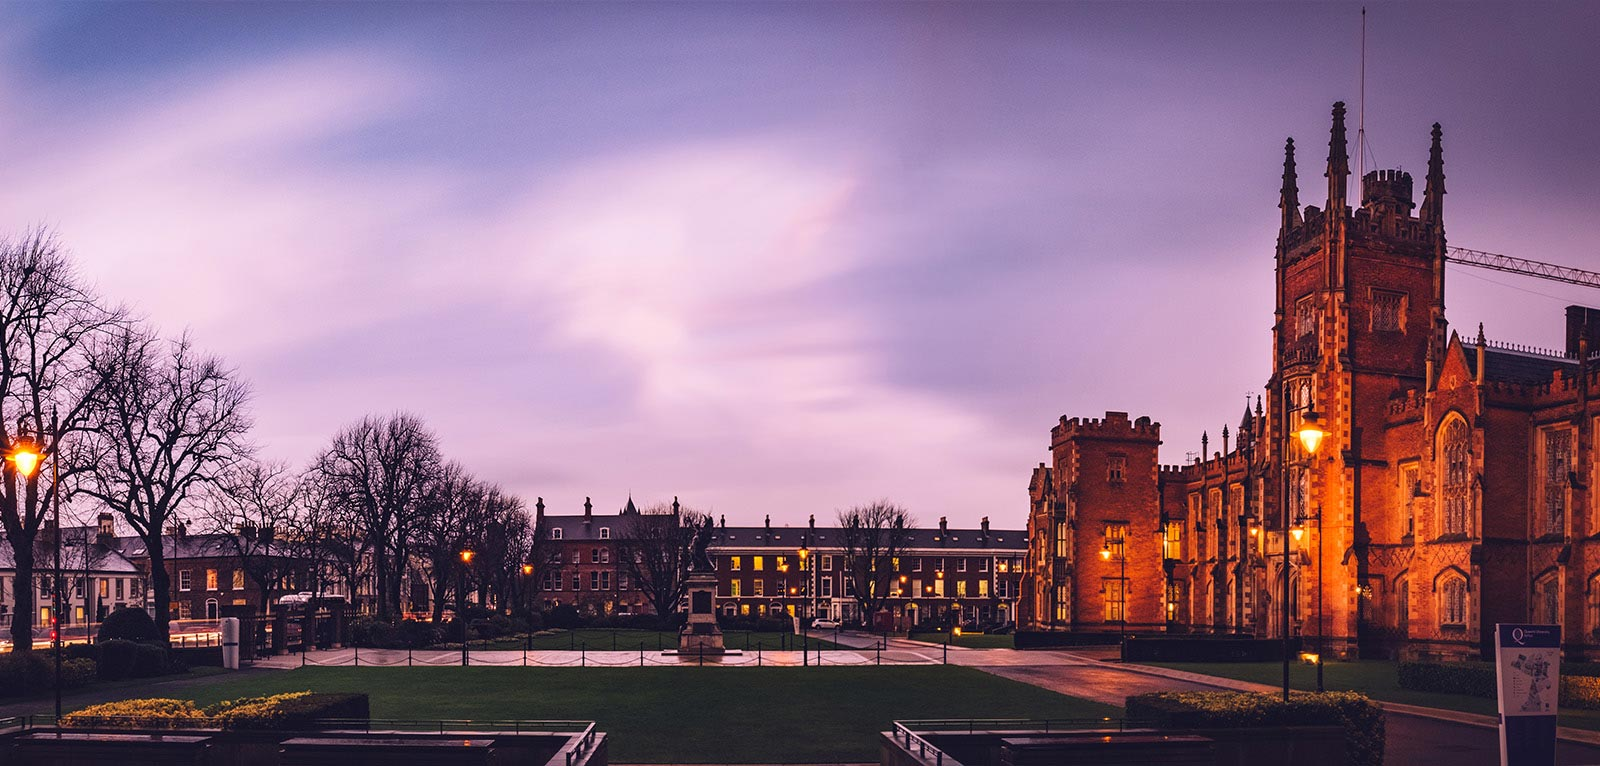
\includegraphics[width=1.1\linewidth]{qub-night.jpg}%{qphys.jpg}
\end{subfigure}
%
\begin{minipage}[t]{.4\textwidth}
\small
\vspace{0.2in}
%\caption{
\centering
{\it
%CTAMOP,\\
%QUB
}

\vspace{-0.1in}




\begin{subfigure}{.9\textwidth}
 \centering

\includegraphics[width=0.8\linewidth]{ctamop.pdf}%{amlogo.jpg}
    \end{subfigure}
%}
\vspace{0.1in}
\begin{subfigure}{.9\textwidth}
 \centering

\includegraphics[width=0.7\linewidth]{epsrc.png}
    \end{subfigure}

\end{minipage}


%\begin{subfigure}{.45\textwidth}
%%\centering
%    \end{subfigure} %
%    \begin{subfigure}{.45\textwidth}
%%       % \centering
%\includegraphics[width=0.25\linewidth]{ksucrest.png}
%    \end{subfigure} %

\end{figure}

%%%%%%%%%%%FUNDING%%%%%%%%%%
%\begin{figure}[h]
%%\colorbox{white}{
%$\begin{array}{lr}
%	
\includegraphics[width=0.5in]{crestq2.png}%{dens-v6-long.jpg} 
%	&
%	
\includegraphics[width=1in, clip=true]{amlogo.jpg}%{dens-v7-long.jpg}
%\end{array}$
%%}
%\end{figure}
%
%
\end{frame}
%
%
%------------------------------------------------
%\fbckg{k-state-seal.pdf}

\fbckg{qubbg3}
%{title}%{k-state-seal.pdf} % Slide background image
\begin{frame}

\begin{center}
{\bf\large R-Matrix theory}
%\\
%Simultaneous measurement allows cancellation of $\tau_A$
\end{center}
\begin{itemize}
\item
Division of space etc...
\end{itemize}
%\tikz{\path[draw=white,fill=white] (-1,1) rectangle (10cm,8.75cm);}
\vspace{-0.2in}


\begin{figure}[h]
%\colorbox{white}{
\centering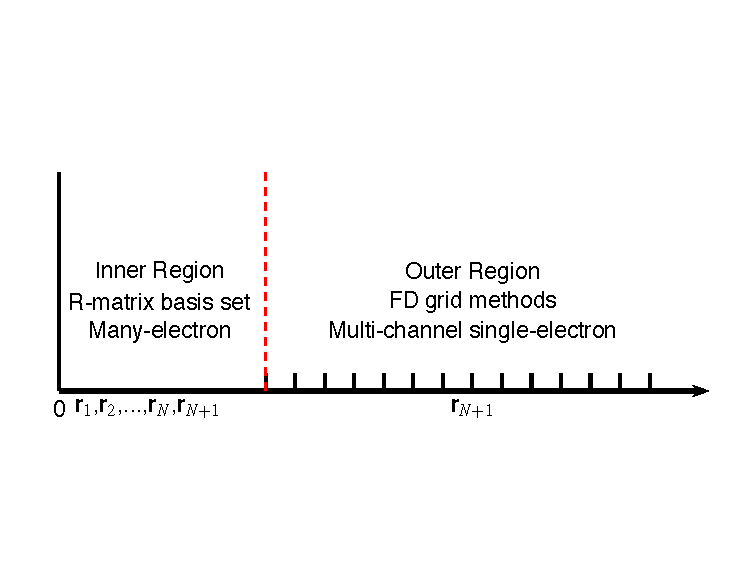
\includegraphics[width=3.5in]{space.pdf}%{potentials}
%}
\end{figure}

%\vspace{-0.8in}
%{\color{black}
%$$
%S(\tau) = \alpha + \beta\cos\left[2\omega\left(\tau-\tau'\right)\right].\hspace{1.4in}\;\;\;\;\;\;\;
%$$
%}
%\vspace{0.8in}
\end{frame}
%------------------------------------------------
\fbckg{qubbg3}
\begin{frame}


\begin{center}
\bf\Large{Inner region}
\end{center}

\small
\begin{itemize}
\item $(N+1)$-electron wavefunction
%\begin{center}
%Can purely nuclear motion show attosecond delays? 
%Need molecule where only permanent dipole transitions occur: HeH$^+$
$$
\small
\Psi({\bf X}_{N+1},t)
= 
\sum_k
C_k(t)
\psi_k({\bf X}_{N+1})
$$
\item Time-dependent coefficients given by
\begin{align}
\frac{d}{dt}{\bf C}(t)
=
-i
\sum_{k'}
{\bf H}(t){\bf C}(t) + i {\bf S}(t)
\nn
\end{align}
\item For linear polarization along $z$-axis, dipole selection rules give $\Delta M_L=0$, $\Delta L=\pm1$ --- dipole matrix takes the form:
\begin{figure}[h]
%\colorbox{white}{
\centering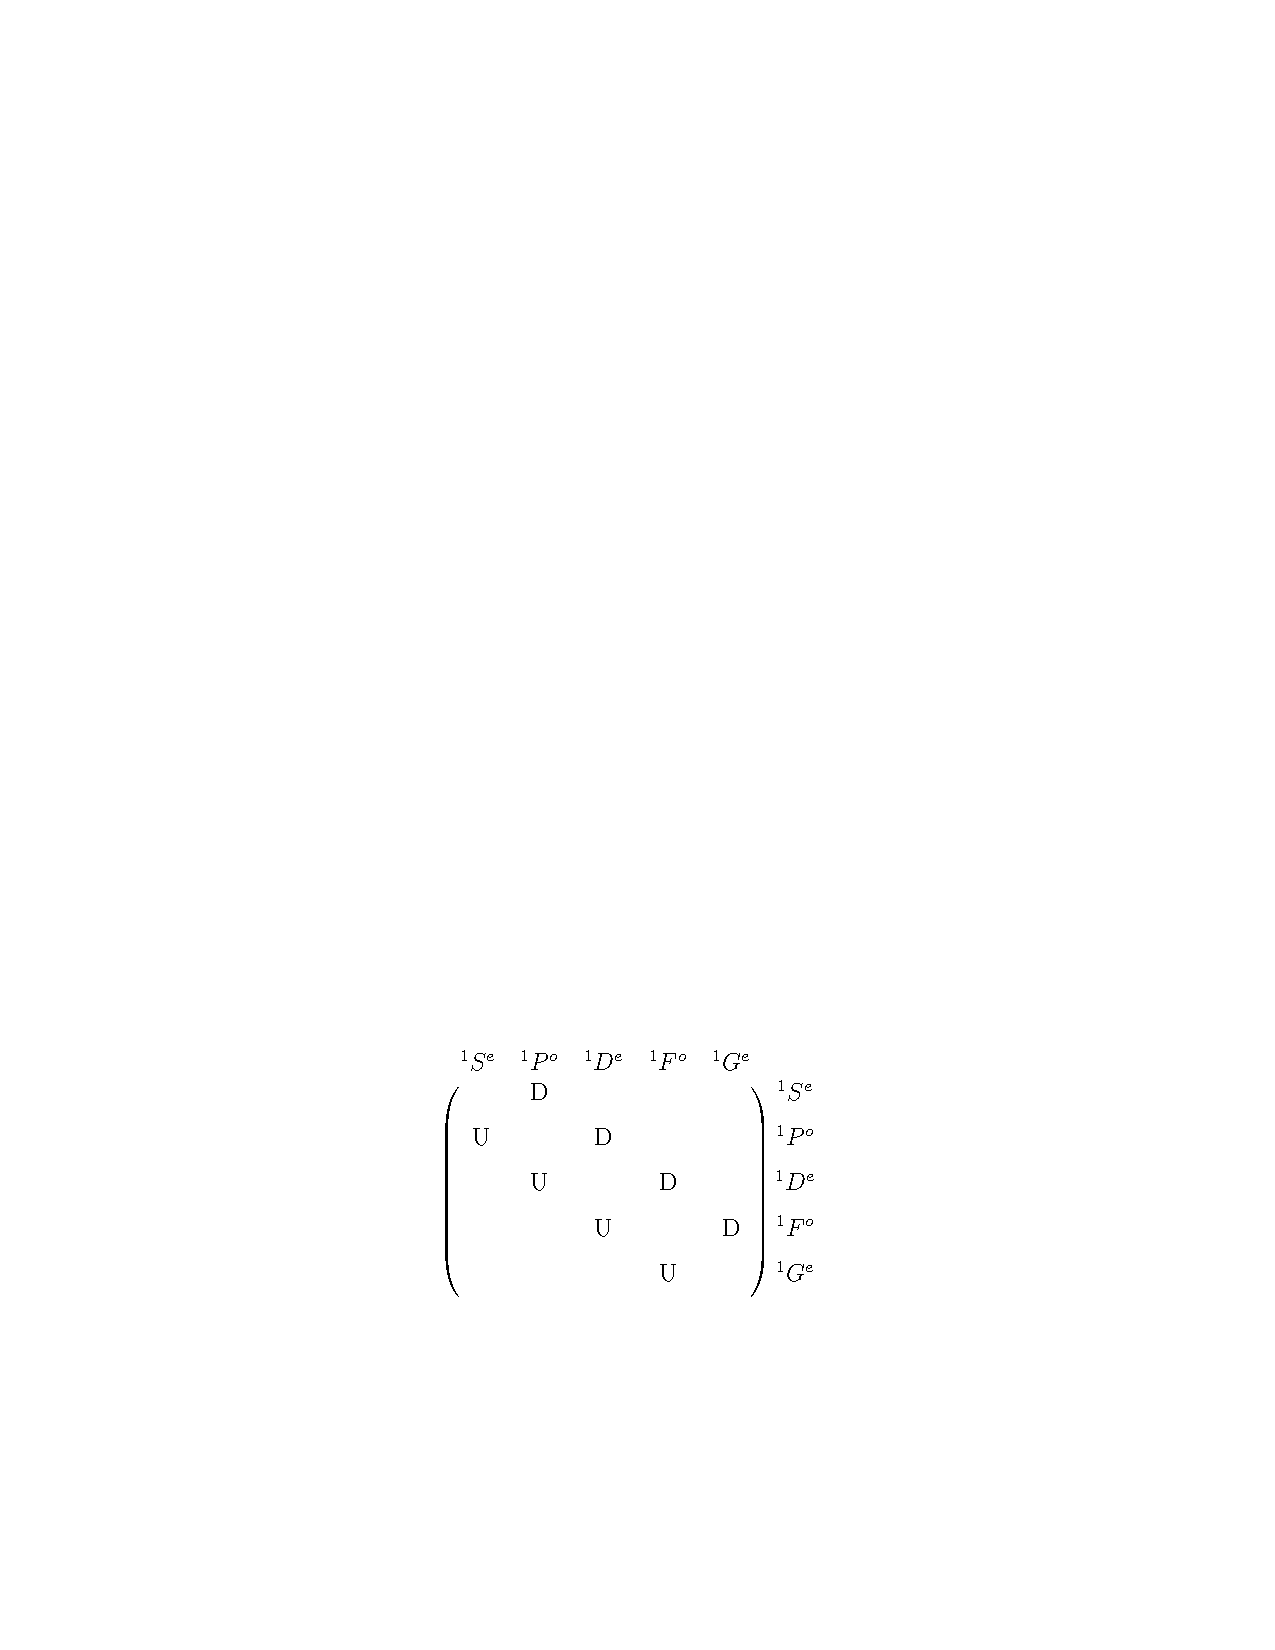
\includegraphics[width=1.5in]{matrixz.pdf}%{potentials}
%}
\end{figure} 

%\end{center}
\end{itemize}

\end{frame}
%
%------------------------------------------------
%\fbckg{k-state-seal.pdf}

\fbckg{qubbg3}
%{title}%{k-state-seal.pdf} % Slide background image
\begin{frame}

\begin{center}
{\bf\large Dipole matrix structure ($L=0,1,2$)}
%\\
%Simultaneous measurement allows cancellation of $\tau_A$
\end{center}
\begin{itemize}
\item
For arbitrary polarization, $\Delta M_L = 0,\pm1$, $\Delta L=0,\pm1$.
\end{itemize}
%\tikz{\path[draw=white,fill=white] (-1,1) rectangle (10cm,8.75cm);}
\vspace{-0.2in}


\begin{figure}[h]
%\colorbox{white}{
\centering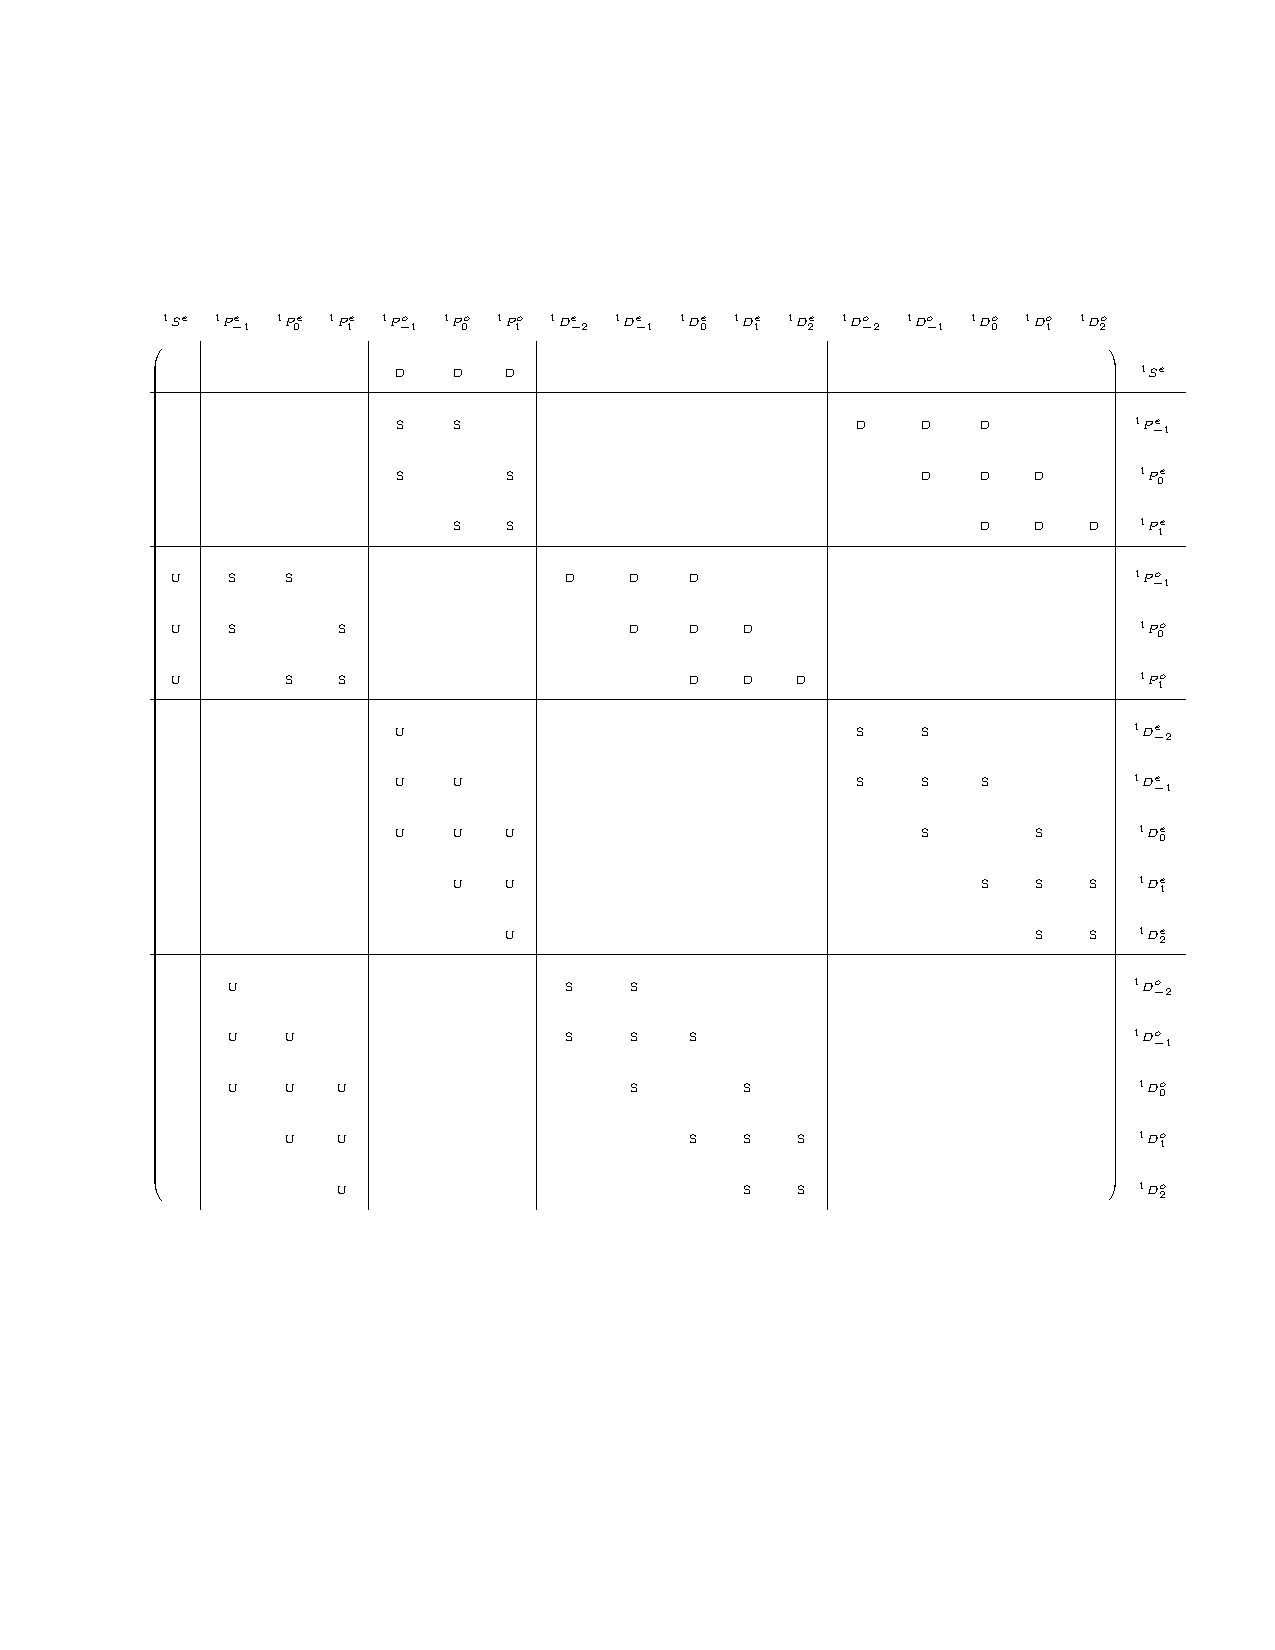
\includegraphics[width=3.5in]{matrix.pdf}%{potentials}
%}
\end{figure}

%\vspace{-0.8in}
%{\color{black}
%$$
%S(\tau) = \alpha + \beta\cos\left[2\omega\left(\tau-\tau'\right)\right].\hspace{1.4in}\;\;\;\;\;\;\;
%$$
%}
%\vspace{0.8in}
\end{frame}

%------------------------------------------------
\fbckg{qubbg3}
\begin{frame}


\begin{center}
\bf\Large{Challenges}
\end{center}

\small
\begin{itemize}
\item Symmetry blocks spread over large number of cores --- at least one core per symmetry block.
\item For $z$-axis polarization, number of $LS\Pi$ symmetry blocks is
$$
N_{LS\Pi} = 2\left(L_{\rm max} + 1\right).
$$ 
\item For arbitrary polarization, number of $LM_LS\Pi$ symmetry blocks is
$$
N_{LM_LS\Pi} = 2\left(L_{\rm max} + 1\right)^2.
$$
\item For strong-field problems, $L_{\rm max} \gg 10$ is typical.
\item Large increase in number of cores allocated to inner region alone.
\end{itemize}

\end{frame}
%
%------------------------------------------------
\fbckg{qubbg3}
\begin{frame}


\begin{center}
\bf\Large{Outer region}
\end{center}

\small
\begin{itemize}
\item $(N+1)$-electron wavefunction
%\begin{center}
%Can purely nuclear motion show attosecond delays? 
%Need molecule where only permanent dipole transitions occur: HeH$^+$
$$
\small
\Psi({\bf X}_{N+1},t)
= 
\sum_p
\overline\Phi_p({\bf X}_N,{\hat r}_{N+1},\sigma_{N+1})
\frac{1}{r}f_p(r,t)
$$
\item Solve coupled-channels radial TDSE for outgoing electron:
\begin{align}
i\frac{\partial}{\partial t}f_p(r,t)
=
\sum_{p'}
\left\langle \overline\Phi_p|H|\overline\Phi_{p'}\right\rangle f_{p'}(r,t).
\nn
\end{align}
$$
p = (\underbrace{\alpha_i L_i M_{L_i}S_i\Pi_i}_{ion}  \;\; \underbrace {l_i m_{l_i}s_i\pi_i}_{electron}   \;\; 
\underbrace{ L M_{L}S\Pi}_{ion+electron})
$$
%\end{center}
\end{itemize}

\end{frame}
%%------------------------------------------------
%\fbckg{qubbg3}
%\begin{frame}
%
%
%\begin{center}
%\bf\Large{Measurements}
%\end{center}
%
%\small
%\begin{center}
%Delay-dependent energy spectra 
%\begin{figure}[h]
%\centering\includegraphics[width=3in]{kplot2.pdf}%{allpots.pdf}%{potentials}
%\end{figure}
%\vspace{-0.1in}
%`Time delay' between diverging wavepackets?
%\end{center}
%
%
%\end{frame}
%
%%%------------------------------------------------
%%\fbckg{qubbg3}
%%\begin{frame}
%%
%%
%%\begin{center}
%%\bf\Large{Second-order perturbation theory}
%%\end{center}
%%
%%\small
%%\begin{itemize}
%%\item Transition matrix element assuming CW laser fields (Eqs. \!(2)--(4)):
%%%\begin{center}
%%%Can purely nuclear motion show attosecond delays? 
%%%Need molecule where only permanent dipole transitions occur: HeH$^+$
%%$$
%%\small
%%T_{a}(k) 
%%= 
%%\mathop{\scalerel*{\SumInt}{\displaystyle\int}}\limits_n 
%%%\displaystyle\SumInt
%%\frac
%%{\langle R_{kl}|r|R_{n1}\rangle  
%%\langle R_{n1}|r|R_{i0}\rangle}
%%{\epsilon_i + \omega_H -\epsilon_n + i\varepsilon}
%%=
%%\langle R_{kl}|r|\rho_{k_{a}1}\rangle 
%%\vspace{-0.1in}
%%$$
%%\item Asymptotic behaviour considered (Eqs.\;(5),(6)):
%%\begin{align}
%%R_{kl}(r)
%% &
%%\xrightarrow[r \to \infty]{} 
%% \sin\left[kr - l\pi/2 + \ln(2kr)/k + \eta_l(k)\right] \nn
%% \\
%%\rho_{k_a1}(r) 
%%&
%% \xrightarrow[r \to \infty]{} 
%% e^{ik_ar - \pi/2 + \ln(2k_ar)/k_a + \eta_1(k_a)}\nn
%%\end{align}
%%\item Relates atomic phase to one-photon scattering phases (Eq.\;(7),(8))
%%\vspace{-0.1in}
%%$$
%%2\omega\tau_I = %\underbrace{u'-P(x)u^2-Q(x)u-R(x)}_{\text{=0, since~$u$ is a particular solution.}}
%%\underbrace{\eta_1(k_e) - \eta_1(k_a)}_{system-dependent} 
%%\;\;+ \;\;\;
%%\underbrace{\varphi_e^{cc}(k) - \varphi_a^{cc}(k)}_{system-independent}
%%$$
%%%\end{center}
%%\end{itemize}
%%
%%\end{frame}
%
%
%
%%------------------------------------------------
%\fbckg{qubbg3}
%\begin{frame}
%
%
%\begin{center}
%\bf\Large{Calculations}
%\end{center}
%
%\small
%\begin{center}
%Total phase (delay, $\tau_I$) is sum of one-photon phase (Wigner delay) and continuum-continuum phase
%\vspace{-0.2in}
%\begin{figure}[h]
%\includegraphics[width=3in]{kplot3.pdf}%{allpots.pdf}%{potentials}
%\end{figure}
%
%
%\end{center}
%
%
%\end{frame}
%
%%------------------------------------------------
%\fbckg{qubbg3}
%\begin{frame}
%
%
%\begin{center}
%\bf\Large{Calculations}
%\end{center}
%
%\small
%\begin{center}
%Wigner term is positive -- energetic electrons escape faster.
%\vspace{-0.2in}
%\begin{figure}[h]
%\includegraphics[width=3in]{kplot3.pdf}%{allpots.pdf}%{potentials}
%\end{figure}
%
%
%\end{center}
%
%
%\end{frame}
%
%%------------------------------------------------
%\fbckg{qubbg3}
%\begin{frame}
%
%
%\begin{center}
%\bf\Large{Calculations}
%\end{center}
%\small
%\begin{center}
%Continuum-continuum part shows opposite behaviour.
%\vspace{-0.2in}
%\begin{figure}[h]
%\includegraphics[width=3in]{kplot3.pdf}%{allpots.pdf}%{potentials}
%\end{figure}
%
%
%\end{center}
%
%
%\end{frame}
%
%%------------------------------------------------
%\fbckg{qubbg3}
%\begin{frame}
%
%
%\begin{center}
%\bf\Large{Calculations}
%\end{center}
%\small
%\begin{center}
%Qualitative agreement with TDSE calculation for H (d).
%\vspace{-0.2in}
%\begin{figure}[h]
%\includegraphics[width=3in]{kplot3.pdf}%{allpots.pdf}%{potentials}
%\end{figure}
%
%
%\end{center}
%
%
%\end{frame}
%
%
%
%
%%------------------------------------------------
%\fbckg{qubbg3}
%\begin{frame}
%
%
%\begin{center}
%\bf\Large{Comparison with experiment}
%\end{center}
%
%\small
%\begin{center}
%\begin{figure}[h]
%\includegraphics[width=3in]{kplot4.pdf}%{allpots.pdf}%{potentials}
%\end{figure}
%
%
%\end{center}
%
%
%\end{frame}
%
%
%
%%------------------------------------------------
%%\fbckg{k-state-seal.pdf}
%\begin{frame}
%
%\begin{center}
%\bf\Large{Summary}
%\end{center}
%\small
%\begin{itemize}
% 
%\item Measured emission from Ar 3s and 3p subshells using RABITT.
%\item Measured energy-dependent atomic phases/time delays.
%\item Derived perturbative expressions for phases/time delays.
%\item Related atomic phase to scattering phase shifts.
%\item Accuracy not well-established through comparisons.
%
%
%\end{itemize}
%
%
%\end{frame}
%
%
%%------------------------------------------------
%\fbckg{qubbg3}
%\begin{frame}
%
%
%\begin{center}
%\bf\Large{Extras}
%\end{center}
%
%\small
%\begin{center}
%\begin{figure}[h]
%\includegraphics[width=3in]{contours2.pdf}%{allpots.pdf}%{potentials}
%\end{figure}
%
%
%\end{center}
%
%
%\end{frame}
%
%
%
%
%%%------------------------------------------------
%%%\fbckg{k-state-seal.pdf}
%%\begin{frame}
%%
%%\begin{center}
%%\bf\Large{Acknowledgements}
%%\end{center}
%%
%%\begin{itemize}
%%
%%\item Brett Esry, Itzik Ben-Itzhak.
%%\item Yujun Wang, Youliang Yu.
%%\item CSGB Division, Office of Science, DOE.
%%
%%\end{itemize}
%%
%%
%%\end{frame}
%%
%%
%%
%%
%%
%
%%------------------------------------------------


\end{document}